% Basic LaTeX template for NE 204 lab report
\documentclass[11pt]{article}

%==============================================================================
%%% Everything between the "="'s is the preamble.
%%% Define packages and meta data here

% Common packages
\usepackage{amsmath}    % Expanded math
\usepackage{amssymb}    % Expanded math symbols
\usepackage{graphicx}   % For images
%\usepackage[version=3]{mhchem} % For nuclide formatting

% All images/figures will be stored in the images folder.
% Specify that here so pdflatex knows where to look for images.
\graphicspath{{./images/}}

% Metadata
\title{Lab2  Digital Signal Processing in HPGe - Timing and
Pulse Shape Analysis}
\author{Yicheng Zhang}
\date{\today}
%==============================================================================

\begin{document}

% Compile metadata from preamble into a nicely-rendered title section
\maketitle

% The *'s next so section/subsection definitions suppresses numbering
\section{Introduction}
\label{sec:intro}

%\begin{figure}
%\includegraphics[scale=0.2]{./1.jpg}
%\end{figure}


Intro:

This lab aims to examine the charge collection and transport properties of a pixelated CdZnTe detector. This Redlen Technologies CZT crystal (crystal number 1498, UCBCZT2) is a 1x1x1 cm3 CZT crystal segmented into nine pixels. Pixels measure 0.75x0.75 mm2 with a 1mm pitch, while the cathode is the full size of the rear face of the crystal. Each pixelated anode is connected an individual built-in pre-amplifier. As two of the pixels are currently not working, we only use the 7 anodes that are and the cathode signals. Thus, we can only use one digitizer (SIS 3302) that has a total of 8 signal inputs with USB interface (SIS 3150) to collect the signal pulses. The correspondence of anode output and port number on the digitizer will be given in the Appendix. The sampling frequency is 100MHz. An optimized trapezoidal filter will be applied to the signal to give spectra for the source signal of Am-241 or Cs-137 [CURRENTLY (11/29) using eventdata trap filter]. Experimental determination of mobility-lifetime product (mutau product) for both electrons and holes in the CZT has been determined using two methods. First is by curve fitting the Hecht relation using photopeak position with different bias voltage; while the second is by assuming constant fractional carrier loss rate per drift distance with different bias voltage. As all of the spectra gathered by illuminating anode with low-energy gammas have poor resolution, we limit our calculation to electron mu-tau product. Additionally, depth of interaction (DOI) has been determined using cathode-to-anode ratio and the time difference method based on the calculated mu-tau product [only CAR implemented 11/29]. Energy calibration was performed and resolution was calculated for both the original spectra and the ones applied with electron trapping compensated spectra. Electron trapping compensated spectra demonstrated significantly poorer resolution, suggesting a problem with the detector or methodology. (mutau will be recalculated based on DOI?)


\section{Methods}
\label{sec:meth}
\subsection{Data collection}
Data collection was performed using NRC-exempt check sources of Am-241 and Cs-137. The UCBCZT2 enclosure was placed cathode-side down on a nonmetallic table, and the check source was centered over the detector face (depending on side). A SIS3302 digitizer and USB interface was used to digitize the pulses with 100MHz sampling rate. Countrates exceeding ~100k/min resulted in buffer overflow. In this case, the detector or source was propped up so as to not alter the x/y location, but to increase the z standoff. The trigger lower bound was set to be 8 in the data collection configuration file to properly capture the whole energy spectrum. 

\subsection{Depth of Interaction}
In this lab, we focus on the use of the cathode to anode ratio (CAR) to determine the depth of interaction (DOI) for individual radiation interaction events. As a secondary priority, we investigate the use of event timing to determine this quantity. In the CAR method, the ratio of the charges collected is indicative of the depth, as the weighting potential due to the cathode is approximately linear across the detector (ignoring contributions by holes). To analyze this quanitity, pulses from anodes 1-7 and the cathode (chn 0) were recorded using the SIS3302, shaped using the built-in trapezoid filter and then run through a coincidence detector to match anode and cathode pulses. A coincidence window length of 1us was chosen based on the rise-time properties of the detector.

Subsequent to event-matching, all anode pulses corresponding to a single cathode pulse (resulting from charge-sharing) were amplitude-summed. The cathode-to-anode ratio was then derived by dividing the cathode pulse amplitude by the summed anode value. The resulting values were then put in a scatter plot. Events with CAR values greater than unity are disregarded, as they are the result of spurious coincidence or extremely poor charge collection. Timing readout [not fully implemented as of 11/29] was achieved by reading in the raw pulse data, finding the peak location using the second derivative. Pulse peaking time for anode and cathode was then adjusted for carrier velocity, and the resulting value was used as a depth-of-interaction metric.

Spectra were generated in several ways. A first-pass spectrum was created by simply histogramming all anode pulses. Alternate spectra were generated by histogramming the anode charge values of all pulses which had a coincident cathode pulse, as well as those that had both cathode coincidence pulses and certain CAR values. This process was also repeated for individual pixels in order to address issues due to differing pixel gain.

Spectrum energy correction was performed on an event-by-event basis by using the CAR depth-of-interaction parameter and a charge collection correction factor. This factor was derived using the Hecht relation (see below). This was used to correct all events with valid interaction parameters (0<x<1), while events with invalid interaction parameters were removed from the data set.

\[Q/Q_0 = {\lambda}_e +{\lambda}_h -{\lambda}_e exp(-(1-x)/{\lambda}_e) - {\lambda}_h exp(-x/{\lambda}_h) \]


\subsection{Curve Fitting}
The peaks in the spectra were fit using a gaussian peak, which is a very rough approximation due to the low-energy tailing present in CZT detectors. This fitting was performed using the SciPy curvefit toolkit.





\clearpage
\section{Results}
\label{sec:res}
\subsection{Cathode to anode ratio spread}

The cathode to anode ratio values found in this investigation were used to attempt to determine depth of interaction and to perform energy correction. DOI values derived from CAR were clustered between 0 and 1, and scatter plots showed features corresponding to peaks (which have been observed in other investigations, cite{Knoll,He}). A small fraction (less than 5 percent) of all C-A scatter points were outside the valid value range, indicating either spurious coincidence or poor charge collection. 

Attempts to correct spectra using CAR and 

[SECTION ON TIMING DOI DETERMINATION]


\begin{figure}[h!]
\begin{center}
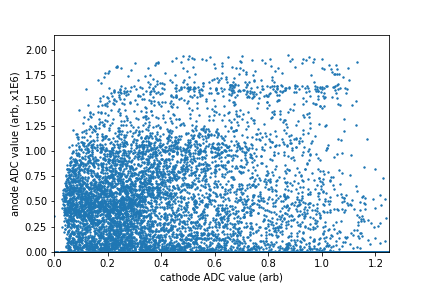
\includegraphics[scale=0.5]{scatter.png}
\caption{This scatterplot shows coincident events as points in cathode-anode space. The distribution of these points shows a strong clustering below cathode values of 4E6 and anode values of 1.2E7. Manually plotting these events shows that these are primarily low-energy events clustered near the anode layer. There is an additional near-horizontal band near an anode value of 1.55E7, which are primarily photopeak events. }
\label{rt}
\end{center}
\end{figure}
\clearpage



\begin{figure}[h!]
\begin{center}
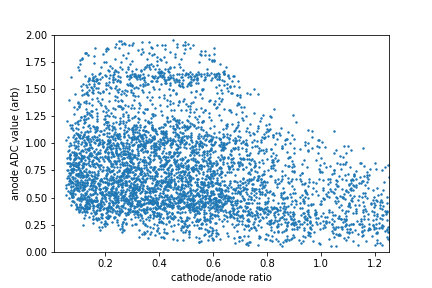
\includegraphics[scale=0.5]{scatter_CAR.png}
\caption{This scatter plot of the anode value versus the cathode/anode ratio demonstrates the banding structure associated with the photopeak clearly near an anode value of 1.55E6. The events with CAR values >1 are mostly spurious coincidence, and will increase in number with larger window settings. Strong clustering is evident at CAR values below .75.}
\label{Ori}
\end{center}
\end{figure}



\begin{figure}[h!]
\begin{center}
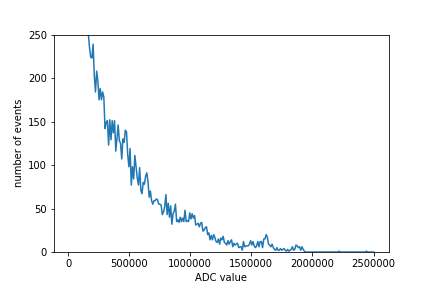
\includegraphics[scale=0.5]{all_anode_pulses.png}
\caption{The energy spectrum associated with all anode events shows extreme low-energy tailing and what appear to be spurious peaks. This spectrum resulted from events occuring at all pixels, and does not exclude anode events with no corresponding cathode pulse. }
\label{400}
\end{center}
\end{figure}


\begin{figure}[h!]
\begin{center}
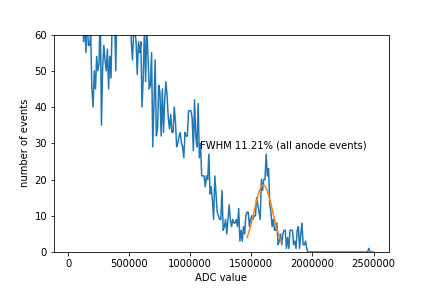
\includegraphics[scale=0.5]{CAR_all.png}
\caption{The energy spectrum associated with all anode events with coincidence shows greatly improved peak resolution, though the number of events has been reduced by an order of magnitude. The fitted FWHM is poor in comparison to most commercial CZT systems, which may be due to depth effects, charge trapping or noise problems.}
\label{400}
\end{center}
\end{figure}


\begin{figure}[h!]
\begin{center}
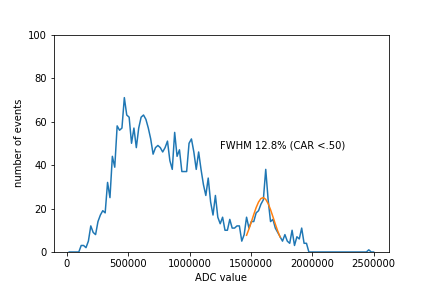
\includegraphics[scale=0.5]{CAR1_all.png}
\caption{Further filtering the coincident anode events by CAR drastically reduces the low-energy background and improves peak FWHM. The fitted FWHM remains poor in comparison to most commercial CZT systems, which may be due to depth effects, charge trapping or noise problems.}
\label{400}
\end{center}
\end{figure}

\begin{figure}[h!]
\begin{center}
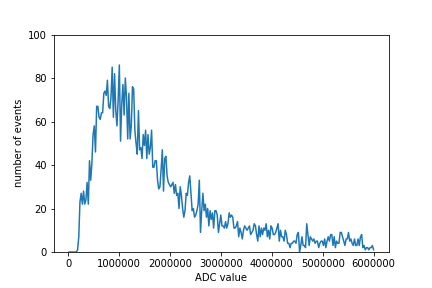
\includegraphics[scale=0.5]{corr_anode_pulses.png}mu
\caption{Attempts to correct the "all coincident pulses" anode data using the Hecht relation was unsuccessful, as is shown in this plot. This may be due to improper mu-tau data or improper correction factor application. This is a focus of future of work.}
\label{400}
\end{center}
\end{figure}

\begin{figure}[h!]
\begin{center}
\includegraphics[scale=0.5]{anodes_px.png}
\caption{Plotting coincident events by anode number demonstrates that pixels 7-8 have significantly different gain and resolution properties. Pixel 1 shows outstanding resolution in comparison to 2-6.}
\label{400}
\end{center}
\end{figure}

\begin{figure}[h!]
\begin{center}
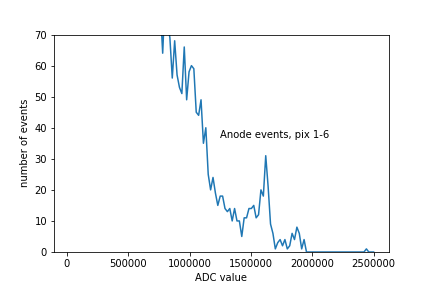
\includegraphics[scale=0.5]{anodes_1_6.png}
\caption{Re-plotting coincident events while excluding anodes 7-8 shows a significant improvement in resolution. This result was durable when tested at different bias voltages and data sets. This will be investigated in the near future.}
\label{400}
\end{center}
\end{figure}




\end{figure}




\section{Discussion}
\label{sec:disc}
\subsection{Quantization error}
[add]


% Bibliography
\bibliographystyle{plain}
% Refers to a bibtex file in the current dir named "references.bib"
\bibliography{references}

\end{document}
